%%%%%%%%%%%%%%%%%%%%%%%%%%%%%%%%%%%%%%%%%%%%%%%%%%%%%%%%%%%%%%%%%%
%%%%%%%%%%%%%%%%%%%% ICML Randomer Forest %%%%%%%%%%%%%%%%%%%%%%%%
%%%%%%%%%%%%%%%%%%%%%%%%%%%%%%%%%%%%%%%%%%%%%%%%%%%%%%%%%%%%%%%%%%

\documentclass{article}

% use Times
\usepackage{times}
% For figures
\usepackage{graphicx} % more modern
\graphicspath{ {/Users/Tyler/LOVEFest/Figures/pdf/} }
%\usepackage{epsfig} % less modern
\usepackage{subfigure} 

% For citations
\usepackage{natbib}

% For algorithms
\usepackage{algorithm}
\usepackage{algorithmic}

% As of 2011, we use the hyperref package to produce hyperlinks in the
% resulting PDF.  If this breaks your system, please commend out the
% following usepackage line and replace \usepackage{icml2016} with
% \usepackage[nohyperref]{icml2016} above.
\usepackage{hyperref}

% Packages hyperref and algorithmic misbehave sometimes.  We can fix
% this with the following command.
\newcommand{\theHalgorithm}{\arabic{algorithm}}

\newcommand{\Real}{\mathbb{R}}
\providecommand{\mc}[1]{\mathcal{#1}}
\providecommand{\mt}[1]{\widetilde{#1}}
\providecommand{\mh}[1]{\hat{#1}}
\newcommand{\T}{^{\ensuremath{\mathsf{T}}}}           % transpose
\newcommand{\argmax}{\operatornamewithlimits{argmax}}
\newcommand{\argmin}{\operatornamewithlimits{argmin}}

% Employ the following version of the ``usepackage'' statement for
% submitting the draft version of the paper for review.  This will set
% the note in the first column to ``Under review.  Do not distribute.''
\usepackage{icml2016} 

% Employ this version of the ``usepackage'' statement after the paper has
% been accepted, when creating the final version.  This will set the
% note in the first column to ``Proceedings of the...''
%\usepackage[accepted]{icml2016}


% The \icmltitle you define below is probably too long as a header.
% Therefore, a short form for the running title is supplied here:
\icmltitlerunning{Randomer Forests}

\begin{document} 

\twocolumn[
\icmltitle{Randomer Forests}

% It is OKAY to include author information, even for blind
% submissions: the style file will automatically remove it for you
% unless you've provided the [accepted] option to the icml2016
% package.
\icmlauthor{Tyler M. Tomita}{ttomita@jhu.edu}
\icmladdress{Johns Hopkins University,
            3400 N Charles St, Baltimore, MD 21210 USA}
\icmlauthor{Joshua T. Vogelstein}{jovo@jhu.edu}
\icmladdress{Johns Hopkins University,
            3400 N Charles St, Baltimore, MD 21210 USA}

% You may provide any keywords that you 
% find helpful for describing your paper; these are used to populate 
% the "keywords" metadata in the PDF but will not be shown in the document
\icmlkeywords{random forest, random projections, machine learning, ICML}

\vskip 0.3in
]

\begin{abstract} 
% The purpose of this document is to provide both the basic paper template and
% submission guidelines. Abstracts should be a single paragraph, between 4--6 sentences long, ideally.  Gross violations will trigger corrections at the camera-ready phase.
\end{abstract} 

\section{Introduction}
\label{intro}

\section{Linear Threshold Forests}

Let $\mc{D}^n=\{(X_i,y_i): i \in [n]\}$ be a given dataset, where $X_i \in \Real^p$ and $y_i \in \mc{Y} = \{\mt{y}_1,\ldots, \mt{y}_C\}$.  A classification forest, $\bar{g}(X; \mc{D}^n)$ is an ensemble of $L$ decision trees, each tree $g^l( X; \mc{D}^l)$  is trained on a (sub)set of the data, $\mc{D}^l \subset \mc{D}^n)$.
% , where $=\{(X_i,y_i): i  \in \mc{S}^l\}$
Linear threshold forests are a special case of classification forests that subsume all of the strategies mentioned above (see Pseudocode \ref{pseudo}).  The key idea of all of them is that at each node of the tree, we have a set of predictor data points, $\bar{X}=\{X_s\}_{s \in \mc{S}^l_{ij}} \in \Real^{p \times S^l_{ij}}$ , where  $S^l_{ij}=|\mc{S}^l_{ij}|$ is the cardinality of the set of predictor data points at the $(ij)^{th}$ node of the $l^{th}$ tree.
We sample a  matrix $A \sim f_A(\mc{D}^n)$, where $A \in \Real^{p \times d}$, possibly in a data dependent fashion, which we use to project the predictor matrix $\bar{X}$ onto a lower dimensional subspace, yielding $\mt{X} = A\T X \in \Real^{d \times S^l_{ij}}$, where $d \leq p$ is the dimensionality of the subspace.  To wit, Breiman's original Forest-IC algorithm can be characterized as a special case of linear threshold forests.  In particular, in Forest-IC one constructs $A$ such that for each of the $d$ columns, we sample a coordinate (without replacement), and put a 1 in that coordinate, and zeros elsewhere. Similarly, Ho's rotation forests construct $A$ from the top $d$ principal components of the data $\bar{X}$ at a given node.  Thus, the key difference in all these approaches is the choice of $f_A$. 


\begin{algorithm}
  \caption{Psuedocode for Linear Threshold Forests, which generalizes a wide range of previously proposed decision forests.} \label{pseudo}
\begin{algorithmic}[1]
  \algorithmicinput 
% \begin{compactitem}
  \State {Data}: $\mc{D}^n = (X_i,y_i) \in (\Real^p \times \mc{Y})$ for $i \in [n]$
  \State {Tree rules}:  $n_{tree}$, stopping criteria, pruning rules, rule for sampling data points per tree, etc.
% \State \textbf{distribution on $[n]$}: $\mc{S}^l \sim f_s$ , where $\mc{S}^l \subset [n]$  is the index set of data points for tree $l$ 
% \item \textbf{Subspace}: $\mc{A}^{p \times d}$
  \State {Distributions on $s \times d$ matrices}: $A \sim f_A(\mc{D}^n)$, for all $s \in [n]$
% \item \textbf{Stoppping criteria}: e.g., a maximal tree depth or minimum number of elements per tree 
% \end{compactitem}
  \State Preprocessing rules
  \algorithmicoutput decision trees, predictions, out of bag errors, etc. 
  \State Preprocess according to rule
  \For{each tree}
  \State Subsample data to obtain $(\bar{X},\bar{y})$, the set of data points to be used in this tree
  \For{each leaf node in tree}
  \State Let $\mt{X} =  A\T \bar{X} \in \Real^{d \times s}$, where $A \sim f_A(\mc{D}^n)$
  \State Find the coordinate $k^*$ in $\mt{X}$ with the ``best'' split
  \State Split $X$ according to whether $X(k) > t^*(k^*)$
  \State Assign each child node as a leaf or terminal  node according to convergence criteria
  \EndFor
  \EndFor
  \State Prune trees according to rule
\end{algorithmic}
\end{algorithm}

The goal of this work is to find a linear threshold forest that posseses many of the properties that RF has, yet is able to find decision boundaries that are less biased by geometrical constraints, in part by changing the distribution $f_A$. The result we call randomer forests (or RerFs for short).
\section{Randomer Forests}

\section{Experimental Results}

% {\footnotesize
% \begin{verbatim}
% dvips -Ppdf -tletter -G0 -o paper.ps paper.dvi
% ps2pdf paper.ps
% \end{verbatim}}

\subsection{Simulations Involving Compressive Signals}

We constructed two synthetic datasets to compare classification performance and training time of RF, RerF, and RotRF:
% \begin{compactenum}

\textbf{Sparse parity} is a variation of the parity problem. The parity problem is a multivariate generalization of the XOR problem and is one of the hardest constructed binary classification problems. In parity, a given sample has a mean whose elements are Bernoulli samples with probability 1/2, and then Gaussian noise is independently added to each dimension with the same variance.  A sample's class label is equal to the parity of its mean. Sparse parity is an adaption of the of the basic parity problem in which the sample's class label is equal to the parity of only the first p* elements of the mean, rendering the remaining p - p* dimensions as noise.

\textbf{Trunk} is a well-known binary classification in which each class is distributed as a p-dimensional multivariate Gaussian with identity covariance matrices \cite{Trunk1979}. The means of the two classes are $\mu_1 = (1,\frac{1}{\sqrt{2}},\frac{1}{\sqrt{3}},...,\frac{1}{\sqrt{p}})$ and $\mu_2 = -\mu_1$. This is perhaps the simplest axis aligned problem, for which random forests should perform exceedingly well. 

For all comparisons, we used the same number of trees for each method to enable a fair comparison. The only parameter tuned was mtry, the number of candidate split directions evaluated at each split node. The left panels of Figure \ref{fig:sim} show two-dimensional scatter plots from each of the three example simulations (using the first two coordinate dimensions). The middle panels show the misclassification rate relative to RF against the number of observed dimensions $p$, for RerF and RotRF. Relative misclassifcation rate was computed as the difference between the misclassification rate of either RerF or RotRF and that of RF. The misclassification rate of RF relative to itself is shown for reference.  The right panels show training time against the number of observed dimensions $p$ for all four classifiers.

\begin{figure}[ht]
\vskip 0.2in
\begin{center}
\centerline{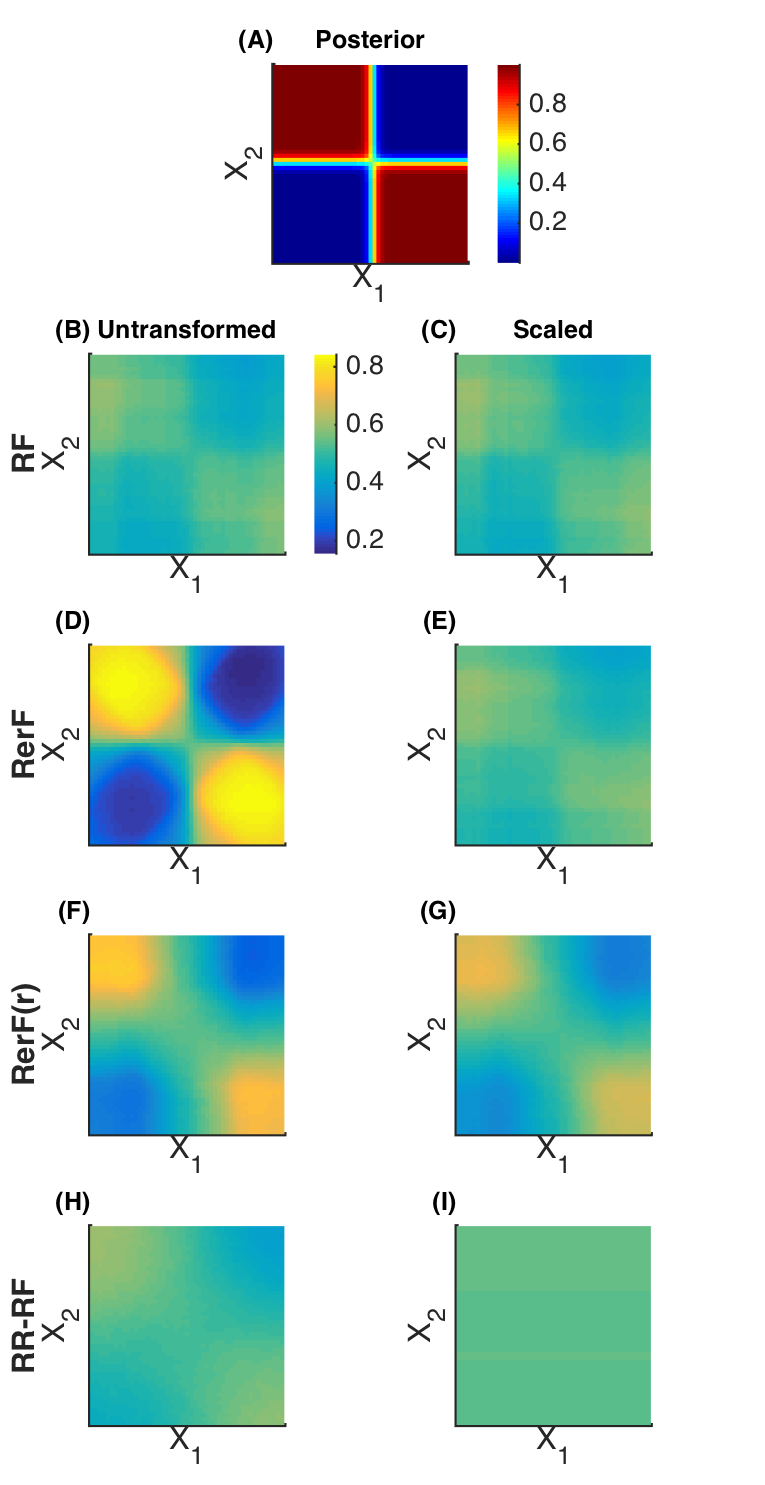
\includegraphics[width=\columnwidth]{../Figures/pdf/Sparse_parity_posteriors}}
\caption{Class posteriors for the sparse parity problem in the first two dimensions. (A): True posteriors. (B) - (D): Posterior estimates for RF, RerF, and RotRF, respectively.}
\label{posteriors}
\end{center}
\vskip -0.2in
\end{figure}

\begin{figure}[ht]
\vskip 0.2in
\begin{center}
\centerline{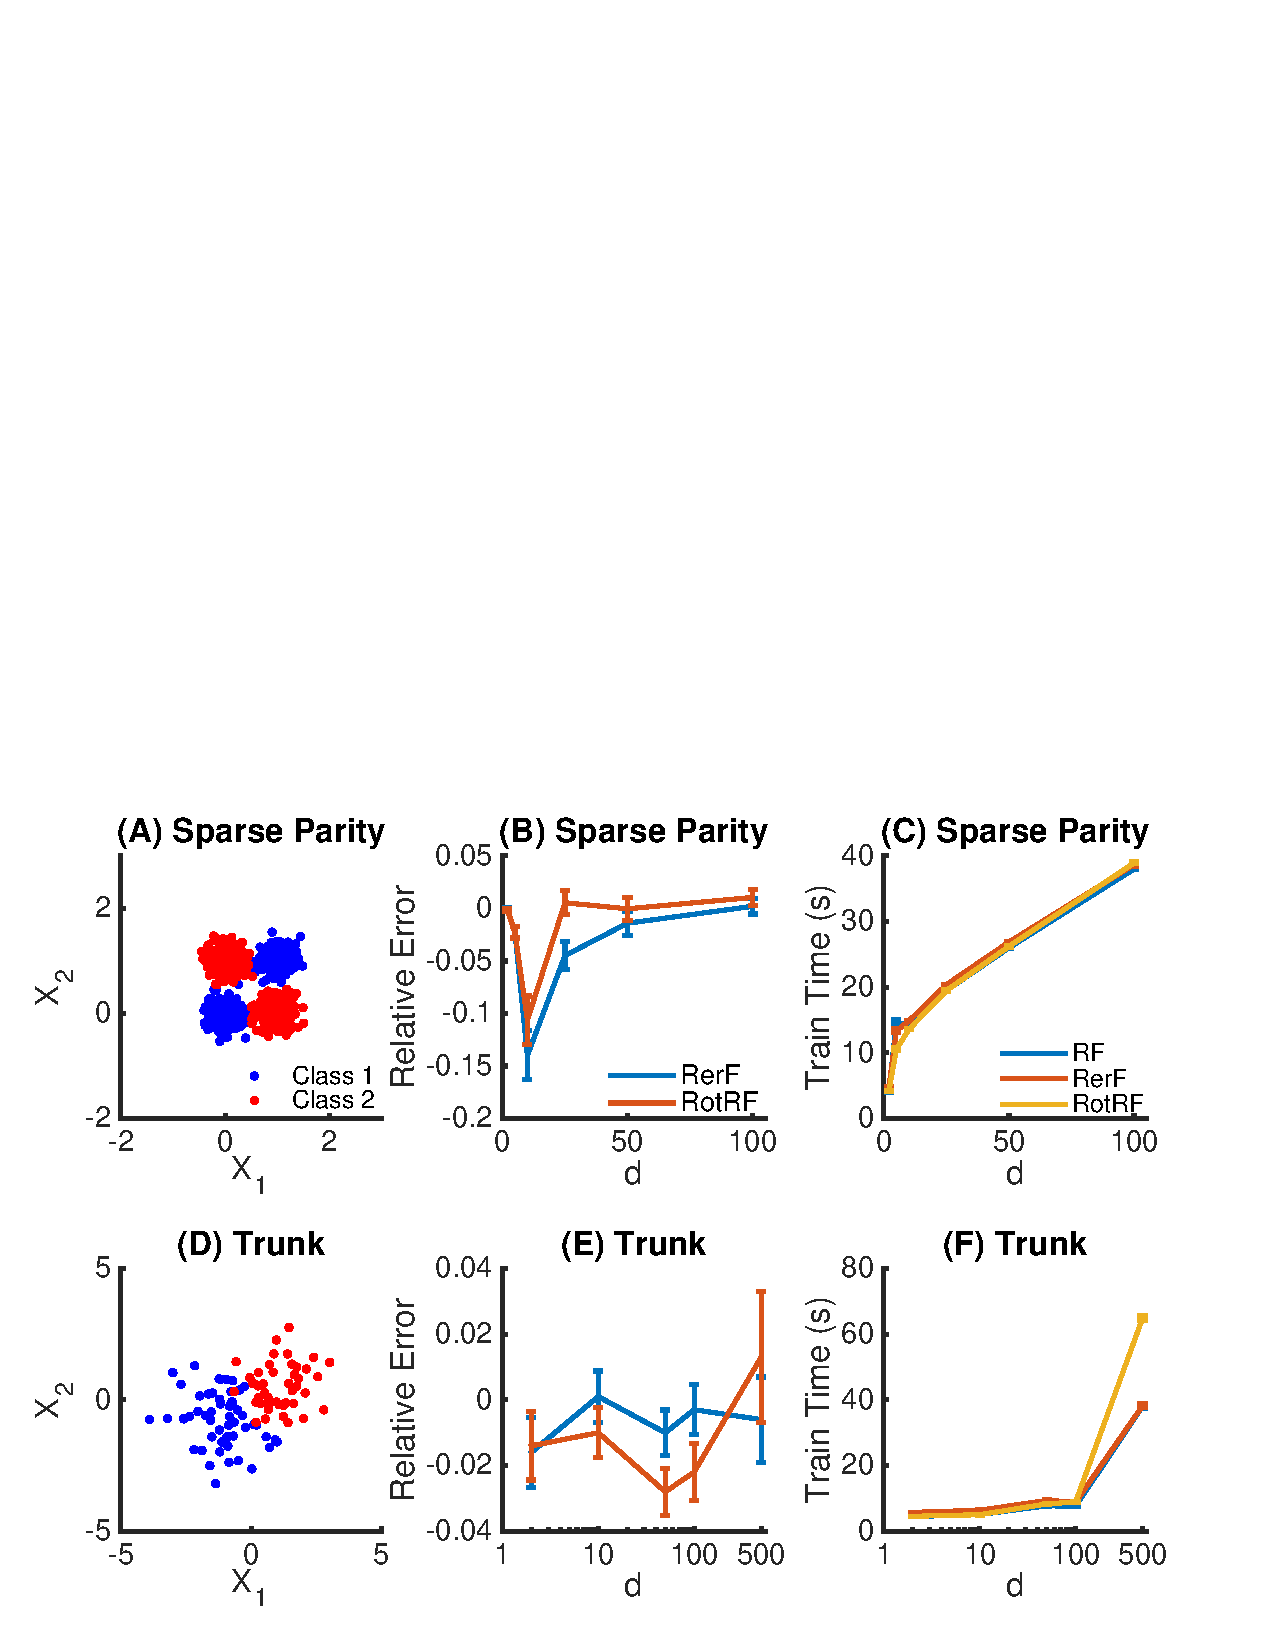
\includegraphics[width=\columnwidth]{../Figures/pdf/Fig2_simulations}}
\caption{Sparse parity (A-C) and Trunk (D-F) simulations. (A) and (D): Scatterplots of sampled points for p = 2. (B) and (E): Error rates of RerF and RotRF relative to RF across different values of p. (C) and (F): Same as (B) and (E) except absolute training time is plotted on the y-axis instead.}
\label{simulations}
\end{center}
\vskip -0.2in
\end{figure}

\subsection{Effects of Transformations and Outliers}

\begin{figure}[ht]
\vskip 0.2in
\begin{center}
\centerline{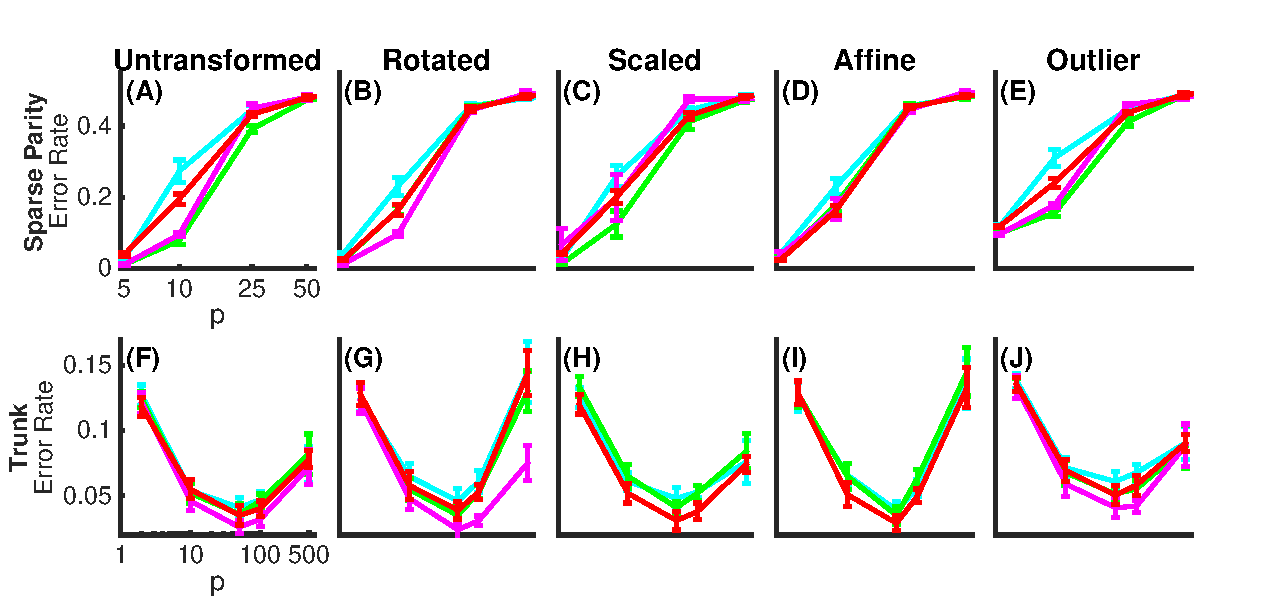
\includegraphics[width=\columnwidth]{../Figures/pdf/Fig3_transformations2}}
\caption{The effects of different transformations applied to the sparse parity (A-E) and Trunk (F-J) simulations on classification performance. Specifically, we consider rotations, scalings, affine transformations, as well as the addition of outliers.}
\label{transformations}
\end{center}
\vskip -0.2in
\end{figure}

\subsection{Benchmark Data}

\begin{figure}[ht]
\vskip 0.2in
\begin{center}
\centerline{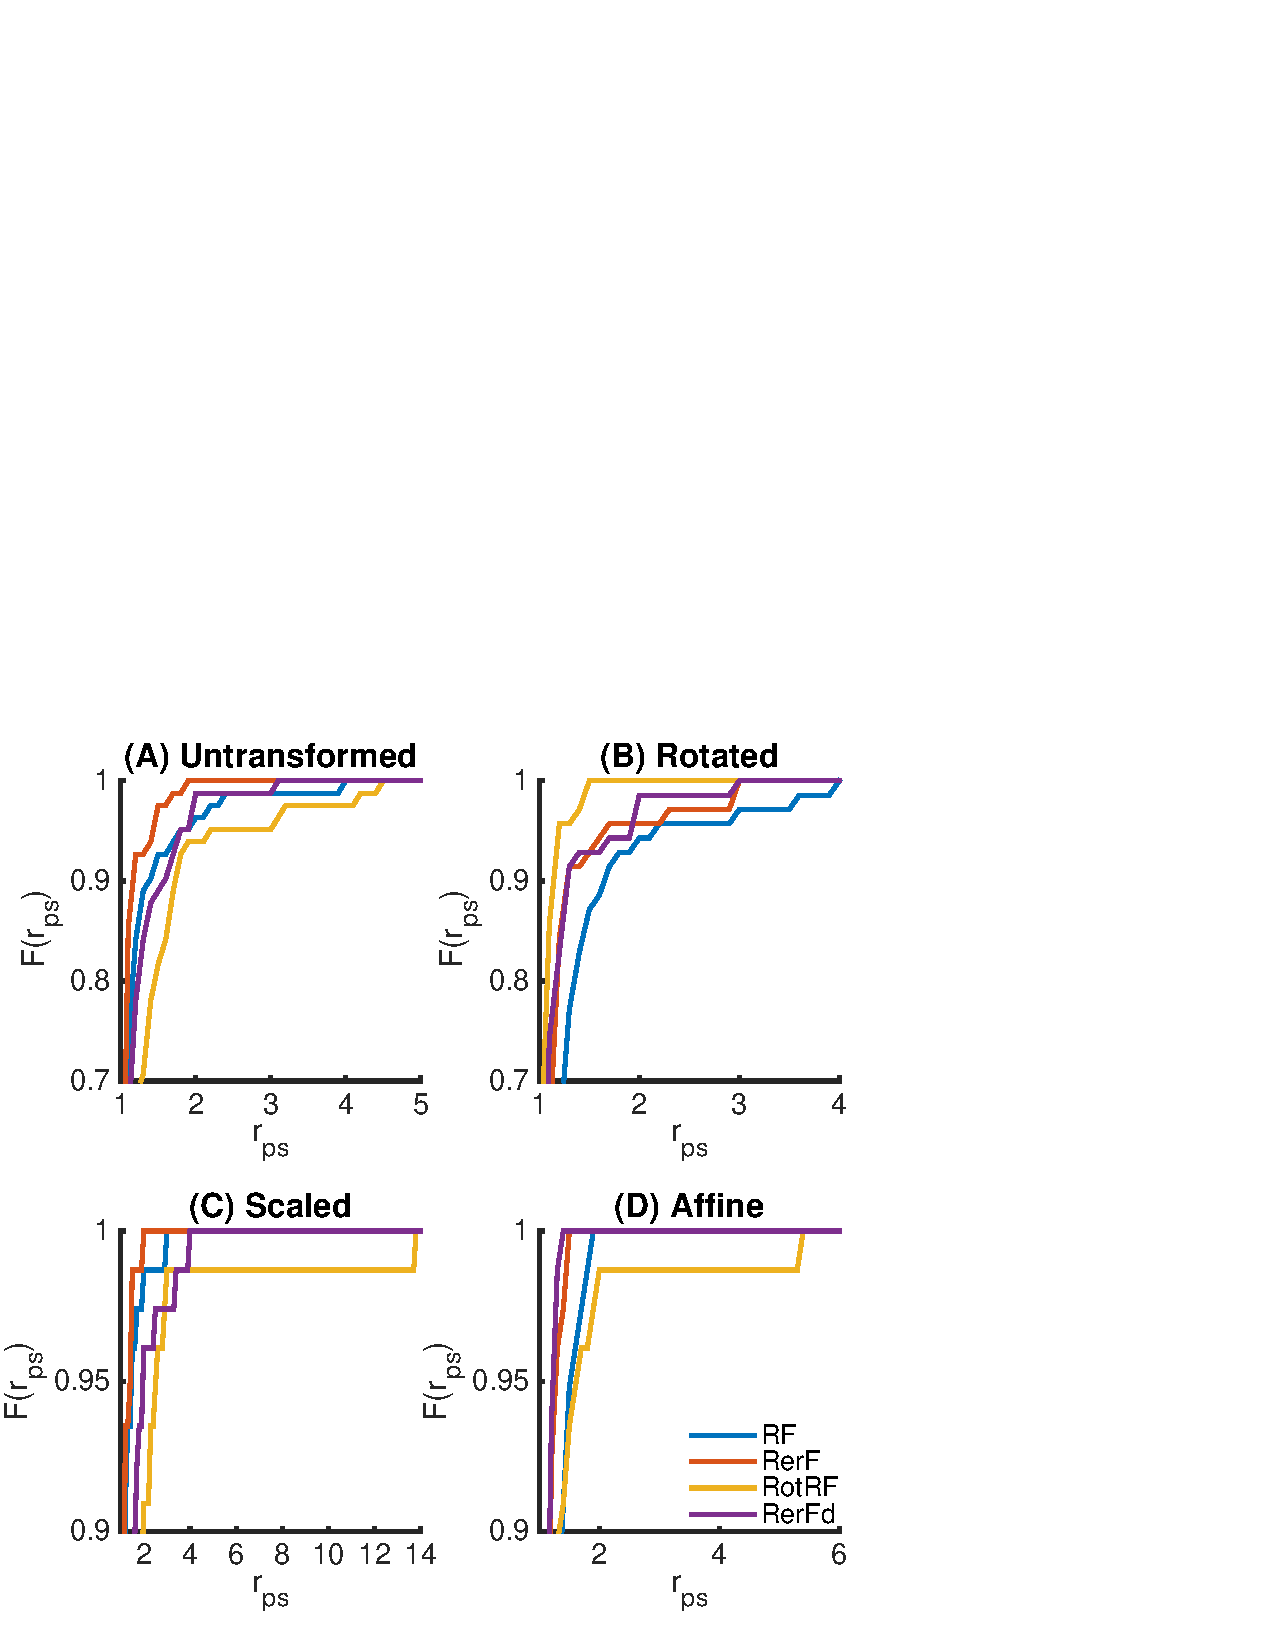
\includegraphics[width=\columnwidth]{../Figures/pdf/Fig4_benchmark}}
\caption{Performance profiles on benchmarks with various transformations applied. AUC denotes the area under the curve.}
\label{benchmark}
\end{center}
\vskip -0.2in
\end{figure}

\subsection{Rank Transforming the Data and Fast Supervised Projections}

\section{Discussion}

\section{Conclusion}

% In the unusual situation where you want a paper to appear in the
% references without citing it in the main text, use \nocite
\nocite{langley00}

\bibliography{example_paper}
\bibliographystyle{icml2016}

\end{document} 


% This document was modified from the file originally made available by
% Pat Langley and Andrea Danyluk for ICML-2K. This version was
% created by Lise Getoor and Tobias Scheffer, it was slightly modified  
% from the 2010 version by Thorsten Joachims & Johannes Fuernkranz, 
% slightly modified from the 2009 version by Kiri Wagstaff and 
% Sam Roweis's 2008 version, which is slightly modified from 
% Prasad Tadepalli's 2007 version which is a lightly 
% changed version of the previous year's version by Andrew Moore, 
% which was in turn edited from those of Kristian Kersting and 
% Codrina Lauth. Alex Smola contributed to the algorithmic style files.  
